\chapter{Artificial Neural Networks}
Neural networks provide a robust method to learn
vector-valued target functions.
% TODO more examples is better
They have effectively been used for a multitude of machine learning domains,
including recognition of handwritten characters
\parencite{LeCun1989}
and
face recognition
\parencite{Cottreil1991},
but also in reinforcement learning
(\cite{anderson1989}; \cite{lin1993}). % inverted pendulum
Both popularity and effectiveness of neural networks can be attributed to
their ability to cope with noisy, real-world data,
as well as being able to approximate any function,
albeit with possibly very large complexity (TODO ref).
% TODO maybe pic
\paragraph{}
In part, they are man's attempt
to model the biology of the brain,
or at least that is where the inspiration came from.
The artificial neural networks we construct
consist of interconnected units,
each taking in real-valued inputs
and outputting a real value,
possibly connecting to multiple other units.
This can be in a directed, feed-forward manner,
but it does not have to be.
Interesting architectures have been discovered
that make use of recurrent connections.
Such architectures will be considered in (TODO link).
To complete the analogy,
the human brain consists of a large amount of densely packed neurons,
approximately $10^{11}$ in total.
Compared to an artificial neuron,
they fire a lot slower
yet still humans are capable of
making incredibly complicated decisions
(or recognitions)
in a matter of less than a second.
This hints at great parallelism,
an attribute that is still important
in the artificial neural networks we construct,
especially in real-life situation reinforcement learning
where decisions must be made swiftly and we cannot wait
for a slower model to finish computing.
While our general purpose machines
are entirely sequential in nature,
parallel hardware has been built specially
for neural network applications.
These are not generally available,
as each domain and even each problem
still require their own specific architectures.
Still, in modern day, many make use
of the parallel capabilities of
Graphic Processing Units (GPUs),
effectively making artificial neural networks even more useful.

The analogy is limited however.
Our use of neural networks draws inspiration from nature
but does not aim to mimic perfectly.
Whereas our neural networks output real values,
biological neurons produce a series of spikes
where both timing and intensity impact the result, % TODO citatie :/?
a phenomenon researchers are still trying to model perfectly.
For now,
we shall content ourselves without the dimension of time.

\section{Building Blocks}
Artificial neural networks are made up of simple elements called units.
Units are connected through directed connections
that are associated with a weight.
These weights are what make up the parameters of the model.
Units are usually divided in layers depending on their function
and location within the network.
Non-input units get their activation signal, i.e. their input,
from some function of the values of the incoming connections
and the weights associated with them.
We call these functions \textit{activation functions}.
They are usually non-linear and play an important role
in how the input value is expressed, or \textit{activated}.

\begin{figure}[h]
\label{fig.neuralnet}
\center
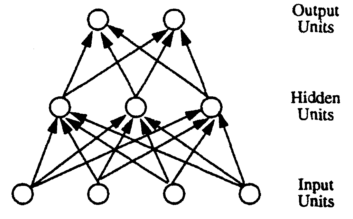
\includegraphics[]{net.png}
\caption{Multi-layer neural network with a single hidden layer.}
\end{figure}

\section{Activation Functions}
\label{sec:activation}

Activation functions are used to transform the output
of a unit in a neural network.
They have a crucial impact on the shape of the output space,
so some care should be taken when deciding on one.

Formally, an activation function $\phi$ will compute

\begin{equation}
  o = \phi (\overrightarrow{w} \cdot \overrightarrow{x})
\end{equation}

where $\overrightarrow{x}$
is the vector of incoming values from other units
and $\overrightarrow{w}$
is the vector of associated weights.

\subsection{Perceptron}
%TODO ref on perceptrons
Activation functions can be linear or nonlinear.
A special kind of unit is the \textit{perceptron},
which outputs either a $-1$ or $1$,
depending on the value of a linear combination of the input:

\begin{equation}
\label{eq.perceptron}
o(\overrightarrow{x}) = \begin{cases}
1 & if \overrightarrow{w}\cdot\overrightarrow{x} > 0 \\
-1 & otherwise
\end{cases}
\end{equation}

\begin{figure}
\label{fig.ml.perceptron}
\center
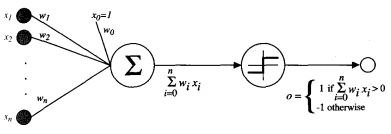
\includegraphics[]{perceptron.png}
\caption{Basic perceptron unit.}
%TODO accredit
\end{figure}

%TODO I have the perceptron img, need to clean and attribute properly
where $\overrightarrow{w}$ denotes the weights of the incoming connection
and $\overrightarrow{x}$ the corresponding incoming values.
This function effectively creates a hyperplane decision surface;
it separates the input space in two.

\subsection{Sigmoid}
\label{sec:sigmoid}
A problem with perceptrons
is that they are not differentiable
in their whole domain.
As I'll explain further down, %TODO ref
differentiability is a useful and ofttimes required attribute.
As a way to circumvent this difficulty of non-differentiability,
the \textit{sigmoid} (denoted $\sigma(x)$) is often used:

\begin{equation}
\label{eq.ml.sigmoid}
\sigma(x) = \frac{1}{1 + e^{-x}}
\end{equation}

\begin{figure}[h]
\center
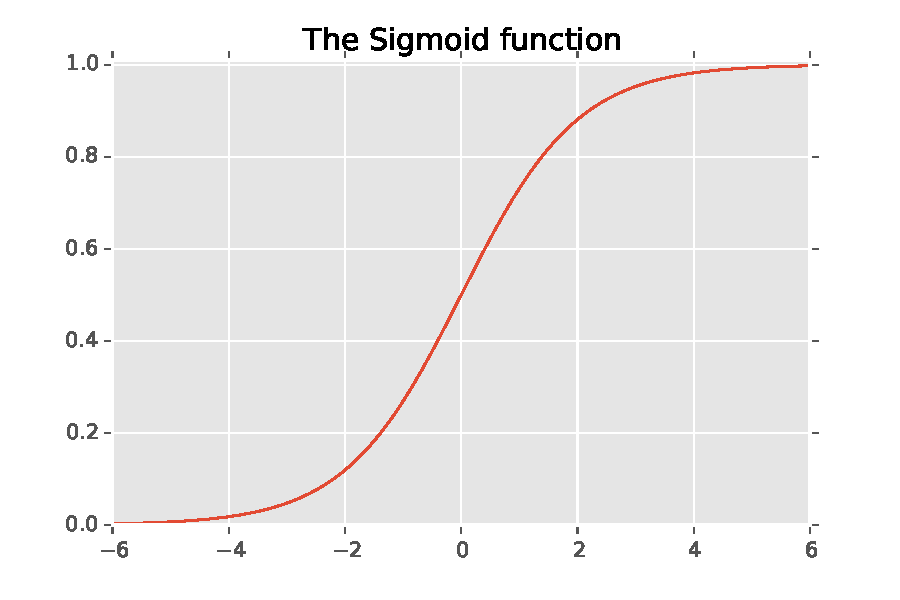
\includegraphics[width=.7\textwidth]{sigmoid.pdf}
\caption{The Sigmoid function}
\label{fig.ml.sigmoid}
\end{figure}

As can be seen on fig \ref{fig.ml.sigmoid},
it has the same tendency as the perceptron activation function
to separate the input space in two
but there is a transition area of uncertainty between the two extremes,
allowing the function to be differentiable in its whole domain.

In practice, the range is normalized between -1 and 1
just like the perceptron.

\subsection{Hyperbolic Tangent}
As a cousin to the sigmoid function, the hyperbolic tangent
deserves mentioning as well.
It bears the same shape as the sigmoid function
since it is really only a stretched
and shifted version.

\begin{equation}
\label{eq.ml.tanh}
htan(x) = \frac{1}{1 + e^{-2x}}+1
\end{equation}

\begin{figure}[h]
\center
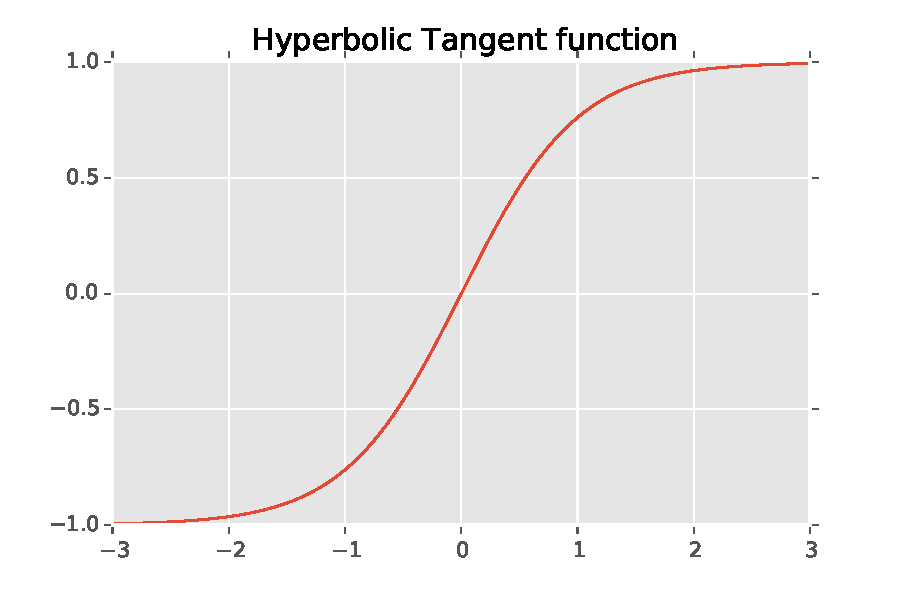
\includegraphics[width=.7\textwidth]{tanh.pdf}
\caption{The Sigmoid function}
\label{fig.ml.htan}
\end{figure}

\section{Rectified Linear Unit}
A fairly recent activation function is the
Rectified Linear Unit, or ReLU for short
\parencite{Nair2010}.

\begin{equation}
\label{eq.relu}
f(x) =
\begin{cases}
0 & \text{for } x < 0 \\
x & \text{for } x \geq 0
\end{cases}
\end{equation}

\begin{figure}[h]
\center
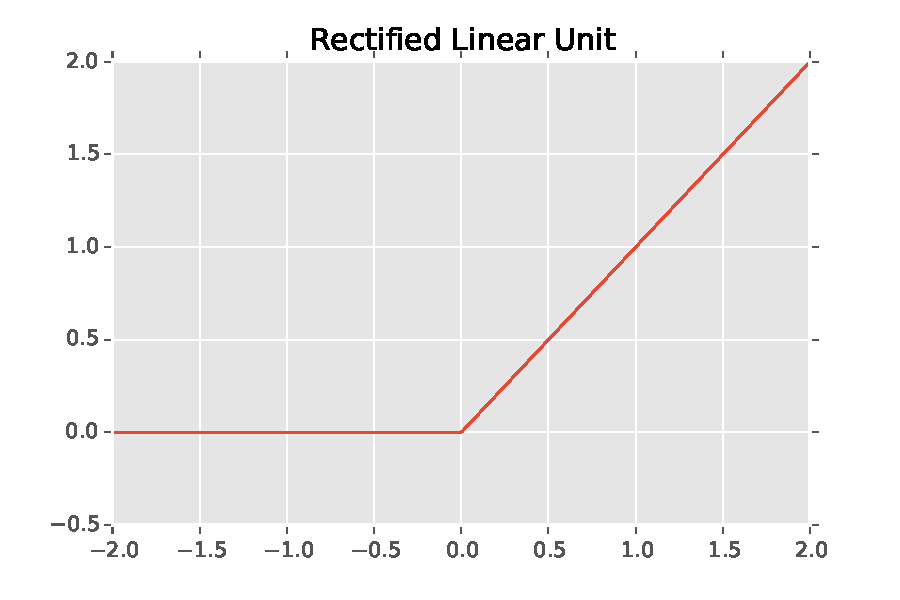
\includegraphics[width=.7\textwidth]{relu.pdf}
\caption{Rectified Linear Unit}
\label{fig.ml.relu}
\end{figure}

While it is very simple in its essence,
it has some important properties
that can be leveraged.
Among the advantages is that anything
below zero is mapped to zero.
This is great for sparse
network activations.
In a scenario with weights initialized
symmetrically (e.g. uniformly) around 0,
only half the neurons will activate.
This sparsity is great for discrimination
and effectively makes training
neural networks faster,
making it especially interesting for
deep learning
\parencite{Y.2015a}.

Linear rectifier functions also help mitigate
the \textit{vanishing gradient} problem %TODO consider ref'ing the vanishing gradient paper
since gradients above zero
are simply propagated.

\paragraph{}
The rectified unit family has gained quite some attention
ever since the first promising results.
Leaky rectified units comprise a subfamily
of functions that are designed to have a non-zero
gradient over their entire domain.
The basic version simply
has a fixed slope below zero
that is kept constant throughout training.

One such variant is the
\textit{Parametric rectified linear unit}
\parencite{He2015a},
a unit with a parametric slope below zero
that can be trained on data.

Another variant is the
\textit{Randomized rectified linear unit}
which has a randomized slope below zero.
The supposition is that the noise
will help prevent overfitting during training,
so the slopes are fixed outside of training.


\section{Gradient Descent and Backpropagation}
\label{sec.backprop}
Earlier we talked about a learning algorithm's error
and even glossed over ways to minimize this error.
In this section we will discuss gradient descent
as a general approach
followed by backpropagation,
a specific gradient descent algorithm
designed to minimize errors
for artificial neural networks.

\paragraph{}
The approaches discussed here
make certain assumptions about
what the algorithm's error looks like
in function of the parameters of the algorithm.
In other words, they make assumptions
about the error surface.

Differentiability is even a requirement, %TODO confirm
meaning the derivative of the error
exists in each point,
so for each combination of algorithm parameters.
This gives rise to smooth surfaces
(though possibly steep)
that do not contain gaps,
such as the one in
Figure \ref{fig:error_surface}.

Despite the requirement,
the methods described here still perform badly
on irregular surfaces:
surfaces where the gradient changes sign often for example,
so surfaces with many local minima.

\begin{figure}[ht]
  \centering
  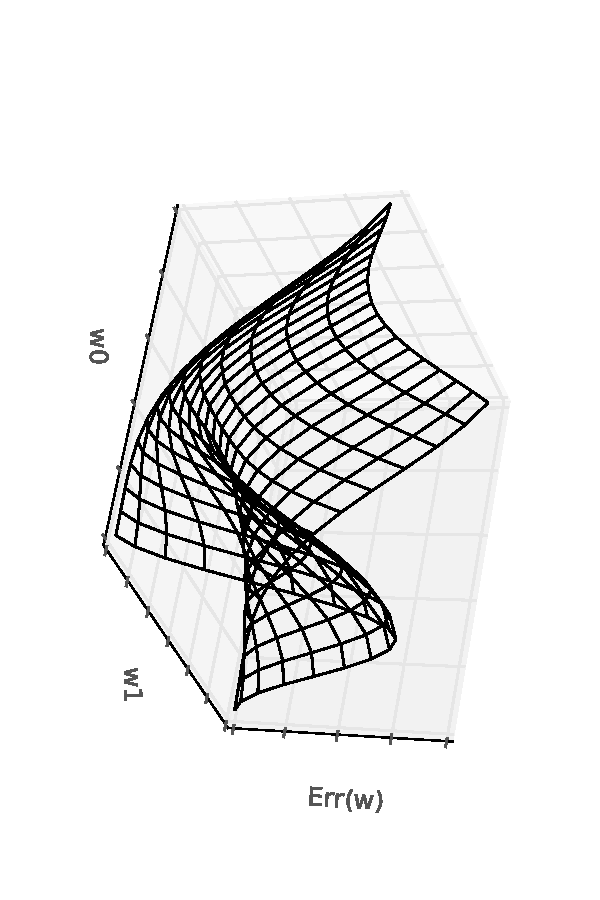
\includegraphics[width=0.7\textwidth]{error_surface2.pdf}
  \caption{Error surface in function of two parameters of the model
  that are to be learned.}
  \label{fig:error_surface}
\end{figure}

\subsection{Gradient Descent}
\label{sub:gradient_descent}

Gradient descent or steepest descent
can be described as the general approach
of moving across an error surface
by following the path with the greatest gradient
- the path with the steepest slope -
downward.
This makes it a greedy algorithm.
Following such a slope
means adjusting the parameters (or weights)
in the direction of the slope.
Figure \ref{fig:gradient_descent}
illustrates what such a walk
would look like on the error surface.

\begin{figure}[ht]
  \centering
  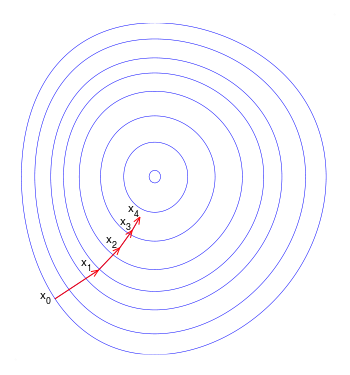
\includegraphics[width=0.5\textwidth]{gradientdescent.png}
  \caption{Gradient descent follows the path with the steepest slope}
  \label{fig:gradient_descent}
  %TODO make own replacement
  %https://en.wikipedia.org/wiki/File:Gradient_descent.svg
\end{figure}

As stated before,
gradient descent requires the derivative of the error E
to exist in the whole domain.
Formally, in function of the weight vector
$\overrightarrow{w}$ of length $n$,
we write the derivative or gradient of E as:

$$
\nabla E(\overrightarrow{w}) = \left(
  \frac{\delta E}{\delta w_0}, \\
  \frac{\delta E}{\delta w_1}, \\
  \dots, \\
  \frac{\delta E}{\delta w_n}, \\
\right)
$$

$\nabla E(\overrightarrow{w})$
is in itself a vector and corresponds to the steepest slope
I described earlier,
with both a size and direction.
Since this gradient describes the steepest
\textit{increase}
of E with respect to $\overrightarrow{w}$,
we need to use the negated gradient
$-\nabla E(\overrightarrow{w})$
to follow the slope downward.

We can now use this for our weight update:

\begin{equation}
\Delta \overrightarrow{w} \leftarrow \overrightarrow{w} - \\
\eta \nabla E(\overrightarrow{w})
\label{eq:gradient_descent}
\end{equation}

We call $\eta$ the learning rate,
useful for tuning the step size of the algorithm.
Smaller values will converge more slowly
while larger ones have the danger of overstepping local minima,
making convergence even slower.
Gradient descent is actually known to 'zigzag'
near convex valleys.
Because of this,
the learning rate is sometimes reduced over time
so the learner is less prone to overstep
and instead settle into minima.


% The method in equation \ref{eq:gradient_descent}
% is also called
% \textit{batch} gradient descent
% because all
\paragraph{}
In order to actually compute the gradient iteratively,
we still need a way to calculate the partial derivations
$\frac{\delta E}{\delta w_i}$.
We still have not defined the error E,
so let us start with that.
For a training data set $D$
and learning algorithm $\hat{f}$,
we define the error $E$ w.r.t. to
$\overrightarrow{w}$ as:

\begin{equation}
  E(\overrightarrow{w}) \equiv \frac{1}{2} \\
  \sum_{(x_i, y_i) \in D}(y_i - \hat{f}(x_i))^2
\end{equation}

As you can see it is close the mean squared error,
with an added advantage that will become clear in a moment.

\paragraph{}
In order to algebraically derive $E$ w.r.t to $w$,
we also need to define the learning algorithm $f$,
which of course plays a key role
in what the error surface looks like.
There are some general computational methods %TODO really cool if I could link any
for computing the gradient near a certain point $x$
in case the algebraic derivation is too hard to calculate
or the calculations are too complex.
However, we will content ourselves with a simpler example
that allows us to perform an algebraic derivation
and calculate the gradient without such methods.

For $f$, we will pick
a simple linear unit that will suffice as an example:

$$
f(\overrightarrow{x};\overrightarrow{w}) = \overrightarrow{x} \cdot \overrightarrow{w}
$$

Finally then, the differentation of $E$:

\begin{equation}
  \begin{split}
    \frac{\delta E}{\delta w_i} &= \frac{\delta}{\delta w_i} \frac{1}{2}
    \sum_{(x_j, y_j) \in D} (y_j - \hat{y}_j)^2 \\
    &= \sum_{(x_j, y_j) \in D}(y_j - \hat{y}_j)
    \frac{\delta}{\delta w_i}(y_j - \overrightarrow{w} \cdot \overrightarrow{x_j}) \\
    &= \sum_{(x_j, y_j) \in D}(y_j - \hat{y}_j)(-x_{ij})
  \end{split}
\end{equation}

with $x_{ij}$ the $i$'th component of $x_j$.
As you can see, the derivation is comfortably easy
because of our choice of the linear unit
and the way the error function is defined.
Other errors but most of all other learning
algorithms can have far less obvious differentiations.

Combining this with \ref{eq:gradient_descent}
gives us the update rule for a specific weight component:

\begin{equation}
  \Delta \overrightarrow{w}_i = \eta \sum_{(x_j, y_j \in D)} \\
  (y_j - \hat{y}_j) x_{ij}
  \label{eq:gradient_descent_update}
\end{equation}

Equation \ref{eq:gradient_descent_update}
describes the gradient descent algorithm for the linear unit.
Each iteration the weight update gets calculated
for all the training examples by computing $\hat{y}_j$
and following \ref{eq:gradient_descent_update},
then summing all weight updates $w_{ij}$
to get $w_i$.
Only once all weight deltas $\Delta w_i$
are calculated should the actual weight vector be updated
(with $\Delta w$ comprised of the individual $w_i$ of course):

\begin{equation}
  \overrightarrow{w} = \overrightarrow{w} + \overrightarrow{\Delta w}
\end{equation}

This then gets repeated until some termination condition is met,
like a sufficiently small error or a desired amount of passes
over the training set.

\paragraph{}
Because first the whole weight update is calculated
with respect to the whole training data set
and only then the weight vector is adjusted,
this vanilla version of gradient descent is also
called \textit{batch gradient descent}.
It can be quite inefficient and downright
impractical for large training sets that do not fit into memory.
For this reason,
the stochastic variant is often used.

\subsection{Stochastic Gradient Descent}
In order to alleviate the problems
with regular stochastic gradient descent's
convergence speed and even tendency to fall
into local minimum pitfalls,
the stochastic approach to gradient descent was devised.

Instead of performing the parameter updates in batch fashion,
parameters are updated incrementally.
This means that for every training sample $(x_j, y_j)$,
$\overrightarrow{w}$
gets updated immediately
and therefore affects the calculation of the next
$\Delta \overrightarrow{w}$.
Stochastic gradient descent basically descends towards the steepest
gradient of the error with respect to a single example.
This makes it much faster than the regular batch version
and allows it to be used for online learning.
It also means that stochastic gradient descent
does not use the true gradient to adjust parameters,
instead it uses some complicated estimate.

It should be ovious that it is computationally cheaper
because it performs a step for every sample
instead of once for the whole sample set,
but it is also good for escaping local minima.
Because of its strange descent behavior,
stochastic gradient descent can actually easily overshoot
shallow local minima, allowing it to find better ones later on.

\paragraph{}
By adjusting $\eta$ to be smaller as compensation,
stochastic gradient descent can be made to approximate
the true gradient arbitrarily closely.
Even better, it has been shown that slowly decreasing
the learning rate, as proposed before,
will allow stochastic gradient descent
to match the convergence behavior
of its batch counterpart.

\subsection{Backpropagation}
We have now laid out the basis for the \textit{backpropagation} algorithm,
a learning algorithm designed for multilayer networks
that are capable of representing even the most nonlinear surfaces.
Backpropagation will allow us to learn the weights of a multilayer network
by minimizing a measure of difference between network output and target output
\parencite{rumelhart1988learning}.
This minimization will be done with gradient descent
and the measure of difference we will employ is

\begin{equation}
  E(\overrightarrow{w}) \equiv \frac{1}{2} \sum_{(x_j, y_j) \in D}
  \sum_{k \in outputs}(y_{kj} - \hat{y}_{kj})^2
\end{equation}

where $y_{kj}$ is the \textit{k}th element of the output value
that corresponds to input sample $x_{j}$,
and $\hat{y}_{j}$ is the network value for $x_{j}$,

so $\hat{y}_{kj}$ corresponds to its $k$th value.
Having the error defined like this allows gradient descent
to minimize the error across all training samples.

\paragraph
The network should have an activation function
as described in Section \ref{sec:activation};
we will refrain from picking a specific example for now
and call this activation function $\phi$.

However, since backpropagation is based on gradient descent,
it has the same requirement of differentiability
of the function in question.
Since the network is made up partly of these activation functions,
we require these be differentiable.
Because of this,
backpropagation can not readily be used with a unit such as the perceptron
because it is not differentiable.

\paragraph{}
In the algorithm, we will need a delta
that signifies how off the network's output is.
The $\delta_n$ described here are actually the negative derivatives of our error
w.r.t. to the network in node n,
but we will not go into a full explanation of how this result was achieved.
I only mention this because this
$-\frac{\delta E}{\delta net_n}$
corresponds closely to the negative gradient we used in gradient descent.

\begin{figure}[h]
  \centering
  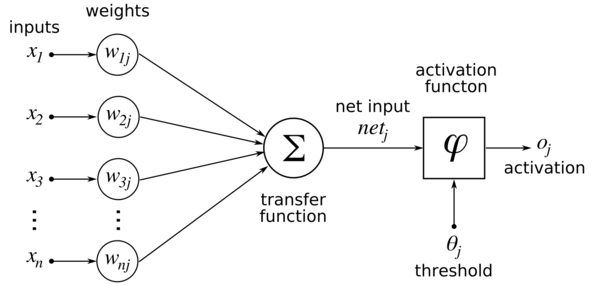
\includegraphics[width=0.8\linewidth]{neuron.png}
  \caption{Overview of different components in a neural network}
  \label{fig:neuron}
\end{figure}

First off, create a neural network
and initialize all network weights.
Initialization can be done in different ways,
according to different distributions,
but a popular standard way of doing things
is to initialize them all according to a small uniform distribution
centered around zero.

Once created, feed the given training sample
through the network, giving $o_k$ as output
for every unit $k$.
The units $o_k$ in the outer layer together
make up $\hat{y}$.

Computing the error term $\delta_k$
for an output unit $k$
and a given training sample
is pretty straightforward:

\begin{equation}
  \delta_k = \psi(o_k) (y_k - \hat{y}_k)
  \label{eq:delta_k}
\end{equation}

with $(y_k - \hat{y}_k)$
simply the difference between the target output and the network output
and $\psi$ the derivative of the activation function $\phi$.
For example, if we were to use
the sigmoid function $\sigma$ (Section \ref{sec:sigmoid}):

\begin{equation}
  \psi(x) = \sigma(x) (1 - \sigma(x))
\end{equation}

and since $o_k$ is calculated by the activation function $\sigma$:

\begin{equation}
  \psi(o_k) = o_k (1 - o_k)
\end{equation}

The $\delta_k$ in \ref{eq:delta_k}
describes the error for an output unit,
but how do we compute the error for a hidden unit,
since a hidden unit has no provided target value?

It turns out it should depend on the error terms
of the units it connects to,
weighted by the weights associated to those connections.
For a hidden unit $h$, write its error term $\delta_h$ as:

\begin{equation}
  \delta_h = \psi(o_h) \sum_{k \in outputs} w_{kh}\delta_k
\end{equation}

where $w_{kh}$ denotes the weight associated to
the connection from unit $h$ to unit $k$.
These are the weights that of course have to be tuned,
so intuitively backpropagation will tune
the responsability or impact of each node for/on the next node,
effectively learning hidden representations about the hypothesis in question.

\paragraph{}
Now that we have defined the error terms for all weights,
we can calculate the weight update
for the weight associated with the connection
from unit $i$ to unit $j$:

\begin{equation}
  \Delta w_{ji} = \eta \delta_j x_{ji}
\end{equation}

Just as with gradient descent,
this can be done until some termination criterion is reached,
be it convergence or amount of iterations.

In the stochastic gradient descent setting of this algorithm,
$\Delta w_{ji}$ would be used immediately to update
$w_{ji}$.
This is how backpropagation is commonly encountered
but one could also choose to employ the batch version
just as was the case with regular gradient descent.
In that scenario,
sum all $\Delta w_{ji}$s
gotten for all examples of the training set
and only then perform weight updates.

In practice this is never done because the approach scales horribly
with training set size.
In fact, backpropagation is usually unleashed on the training set multiple times
in order to converge to a local minimum,
seeing every sample more than once.

\subsubsection{Momentum}
A common extension to backpropagation is momentum.
Every weight update,
you carry over some of the weight update from last iteration:

\begin{equation}
  \Delta w_{ji}(t+1) = \eta \delta_j x_{ji} + \\
  \alpha \Delta w_{ji}(t)
  \label{eq:momentum}
\end{equation}

We call $\alpha$ in \ref{eq} the \textit{momentum}.
It is aptly named after the physical property
and describes how a moving object needs a
larger force to be applied (or for longer)
in order for it to come to a standstill,
the larger the momentum
(and analogously for getting up to speed,
though we conveniently ignore that).

As a result,
a high momentum will keep the weight vector
rolling in the same direction in flat regions
and even roll up small slopes thanks to momentum
accumulated previously,
great for escaping local minima
overcoming flat plateaus.

As an extra,
convergence is sped up
because regions with unchanging downward slopes (negative gradients)
will accumulate a lot of speed.
